\chapter{高速非均匀流场的机理研究}
对于高速流场而言,这种介质非均匀的折射率分布决定了光信号的传输特性,同时流场的物理结构能够通过密度的分布情况来描述,可以说流场密度及折射率的分布是研究气动光学效应的基本核心,而力学中的质量守恒原理及连续方程确定了密度和折射率之间的直接链接关系,因此,如何比较准确地计算高速非均匀流场的密度成为了定量研究气动光学效应的关键,目前能够通过计算流体力学的理论结合数值模拟的方法来求解流场参数。
\section{流体运动基本理论}
流体力学是一门主要通过理论分析、实验及数值计算等方法来研究流体宏观运动规律的学科,它在航空航天领域得到了广泛应用。通过理论分析,科学家们建立了流体运动普遍遵守的运动方程,即Navier-Stokes方程组(简称N-S方程组),并且针对基础研究建立了理想流体等各种简化的流体模型,给出了流体运动方程组的详细的计算方法,为流体力学的研究奠定了基础。

学者们根据经典力学的质量守恒定律、牛顿定律以及能量守恒定律,建立了流体运动的基本方程,他们假设在流场中取一个随机的正六面体微元,长宽高为别为$\Delta x,\Delta y$和$\Delta z$,体中心的坐标为$(x,y,z)$,根据欧拉理论,不同时间内不同的流体占据了该微元,流体不断出入边界,这样,选取的微元就和周围的流体之间有了相互作用,从而产生能量、质量等的交换,因此,对微元建立的运动方程就能够代表整个流体的运动方程。例如可以将t时刻在$(x-\Delta x/2,y,z)$处的物理量$\Phi(x-\Delta x/2,y,z,t)$表示为式\eqref{eq:lizi}所示。
\begin{equation}
\Phi(x-\frac{1}{2}\Delta x,y,z,t)=\Phi(x,y,z,t)-\frac{\partial\Phi(x,y,z,t)}{\partial x}\cdot\frac{1}{2}\Delta x
\label{eq:lizi}
\end{equation}

根据质量守恒定律,单位时间内流入、流出微元边界的净质量应该和微元内的流体质量对时间的变化率相等,如式\eqref{eq:lianxu1}所示。
\begin{equation}
\frac{dm}{dt}=\dot{m}=\rho u\cdot\mathbf{A}
\label{eq:lianxu1}
\end{equation}
式中$\rho$为流体中心密度,$\dot{m}$为质量流量,$u$为流体运动速度,$\mathbf{A}$为流体面的面积。

微元的质量$m$等于密度$\rho$与体积$\Delta x\Delta y\Delta z$的乘积,微元体积可以认定为恒定值,仅有流场的密度在变化,则在微元体内的质量对时间的变化率可以表示为式\eqref{eq:zlsj}所示。
\begin{equation}
\frac{\partial(\rho\Delta x\Delta y\Delta z)}{\partial t}=\frac{\partial\rho}{\partial t}\Delta x\Delta y\Delta z
\label{eq:zlsj}
\end{equation}

将式\eqref{eq:lianxu1}、式\eqref{eq:zlsj}应用到正六面体微元时,假定流体从负轴流向正轴,质量流出为负,流入为正,且不考虑回流,则正六面体的对立面一进一出,令沿$x_i$方向速度为$u_i$,那么在$x_i$方向上流入的质量流量为$[\rho u_i-[\partial(\rho u_i)/\partial x_i]\cdot\frac{1}{2}\Delta x_i]\Delta y_i\Delta z_i$,可以推导出可压缩流体的质量守恒方程即连续方程\eqref{eq:lianxu}。
\begin{equation}
\frac{\partial\rho}{\partial t}+\frac{\partial(\rho u_i)}{\partial x_i}=0
\label{eq:lianxu}
\end{equation}

如果假定流体不受外力,忽略质量力对其的影响,微元只受到压力$p$及粘性应力作用,考虑$x$方向上受力总和为:
\begin{equation}
(-\frac{\partial p}{\partial x}+\frac{\partial\tau_{xx}}{\partial x}+\frac{\partial\tau_{yx}}{\partial y}+\frac{\partial\tau_{zx}}{\partial z})\Delta x\Delta y\Delta z
\label{eq:shouli}
\end{equation}
式中,$p$为压力,$\tau_{ij}$为$ij$面上的应力张量在$j$方向上的分量,$i$取$x,y,z$,$j$取$x$。$\tau_{ij}$可以通过广义牛顿粘性定律用式\eqref{eq:nxzl}表示:
\begin{equation}
\tau_{ij}=2\mu\Bigg[\frac{1}{2}\Big(\frac{\partial u_i}{\partial x_j}+\frac{\partial u_j}{\partial x_i}\Big)-\frac{1}{3}\frac{\partial u_k}{\partial x_k}\delta_{ij}\Bigg]
\label{eq:nxzl}
\end{equation}
式中, $\delta_{ij}$为二阶单位张量的分量,$\mu$为粘性系数。粘性应力张量的所有分量都可以用流体速度分量配合粘性系数表示。

利用式\eqref{eq:shouli}对该微元应用动量定理,即有:
\begin{equation}
\rho\frac{\mathbf{D}u}{\mathbf{D}t}=-\frac{\partial p}{\partial x}+\frac{\partial\tau_{xx}}{\partial x}+\frac{\partial\tau_{yx}}{\partial y}+\frac{\partial\tau_{zx}}{\partial z}
\label{eq:dlfc}
\end{equation}

将质量守恒方程\eqref{eq:zlsj}代入式\eqref{eq:dlfc},并且通过欧拉方法对公式\eqref{eq:dlfc}进行化简,可以得到在流体中使用最为广泛的动量方程\eqref{eq:dongliang}。
\begin{equation}
\frac{\partial(\rho u_i)}{\partial t}=-\frac{\partial p}{\partial x_i}-\frac{\partial(\rho u_iu_j)}{\partial x_j}+\frac{\partial \tau_{ij}}{\partial x_j}\label{eq:dongliang}
\end{equation}

根据能量守恒定律可以知道,在单位时间内周围流体对微元做的功加上周围流体传递给微元的热量净增加之和与微元内总能量对时间的变化率相等,如果令$\mathbf{E}$代表总能量,则总能量对时间的变化率可以表示为式\eqref{eq:nlgr}。
\begin{equation}
\rho\Delta x\Delta y\Delta z\frac{\mathbf{DE}}{\mathbf{D}t}
\label{eq:nlgr}
\end{equation}

能量的交换与力的做功有关,微元单位面积内的流体压力$p$以及粘性应力$\tau_{ij}$对微元做的功应该等于作用力与力方向上的速度之积,分别对三个坐标轴方向计算,累加后可以得出周围流体对微元所做的功可以表示为式\eqref{eq:nlzg}。
\begin{equation}
\Big[-\frac{\partial(pu_i)}{\partial x_i}+\frac{\partial(u_j\tau_{ij})}{\partial x_i}\Big]\Delta x\Delta y\Delta z
\label{eq:nlzg}
\end{equation}

如果忽略系统与外界的热量交换,仅考虑系统内部的热传递,那么根据傅里叶传导定律,周围流体传递给微元的热量能够表示为式\eqref{eq:chuandao}。
\begin{equation}
\mathbf{q}=-\kappa\nabla T
\label{eq:chuandao}
\end{equation}
式中,$\mathbf{q}$为热通量矢量,$\kappa$为热传导系数,导热系数$\kappa$可以用定压比热$C_p$、粘性系数$\mu$以及普朗特数$Pr$(气体通常取0.72)联合表示,如式\eqref{eq:daore}所示。
\begin{equation}
\kappa=\frac{\mu C_p}{Pr}
\label{eq:daore}
\end{equation}

在此可以参考对于动量方程的分析方法,令流入为正,流出为负,对$x,y,z$方向上分别计算,并进行累加后,可得出周围流体传递给微元的净热量应该为:
\begin{equation}
\Big[\frac{\partial}{\partial x}(\kappa\frac{\partial T}{\partial x})+\frac{\partial}{\partial y}(\kappa\frac{\partial T}{\partial y})+\frac{\partial}{\partial z}(\kappa\frac{\partial T}{\partial z})\Big]\Delta x\Delta y\Delta z\Rightarrow\frac{\partial}{\partial x_i}(\kappa\frac{\partial T}{\partial x_i})\Delta x\Delta y\Delta z
\label{eq:nlrl}
\end{equation}

根据能量守恒定律,式\eqref{eq:nlgr}即可等于式\eqref{eq:nlzg}加上式\eqref{eq:nlrl},同样参考动量方程简化方法,利用欧拉方法对其进行化简,即可得到流体的能量方程\eqref{eq:nengliang}。
\begin{equation}
\frac{\partial(\rho E)}{\partial t}=-\frac{\partial[(\rho E+p)u_i]}{\partial x_i}+\frac{\partial(u_j\tau_{ij})}{\partial x_i}+\frac{\partial}{\partial x_i}\Bigl(\kappa\frac{\partial T}{\partial x_i}\Bigr)
\label{eq:nengliang}
\end{equation}

至此,连续方程\eqref{eq:lianxu}、动量方程\eqref{eq:dongliang}以及能量方程\eqref{eq:nengliang}三个方程组成了流体运动方程组(N-S方程组),这是至今为止工程应用中长期用来描述流场运动的基本方程,到目前为止该方程求解的简单工程结果与一些湍流流场的实验数据比较一致,因此,本文关于高速流场的讨论、数值模拟计算等都是基于高速飞行器周围的非均匀流场满足N-S方程组的基础之上进行的。

由于本文讨论的高速流场的介质是空气,能够近似假设为完全气体,因此可以引入气体的状态方程及粘性系数方程以对N-S方程组进行补充。一般来说,流体的粘性系数$\mu$与流体温度有关,与压力基本没有关系,对最广泛的完全气体,它的动力粘性系数大都用Sutherland的经验公式\eqref{eq:nianxing}表示。
\begin{equation}
\frac{\mu}{\mu_0}=\frac{T_0+B}{T+B}(\frac{T}{T_0})^{\frac{3}{2}}
\label{eq:nianxing}
\end{equation}
式中,$T$为气体温度,$T_0$为参考温度,$\mu_0$为参考粘性系数,$B=110.4K$,一般当$T_0=273K$时,$\mu_0=1.176\times 10^{-5}N\cdot S/m^2$。

当考虑介质是完全气体时,它的热力学参量满足方程组:
\begin{subequations}
\label{eq:zhuangtai1}
\begin{align}
p=\rho RT\\
e_0=C_\upsilon T\\
\frac{C_p}{C_\upsilon}=\gamma
\end{align}
\end{subequations}
式中,$R$为气体常数,$e_0$为单位质量流体的内能,$C_\upsilon$为定容比热,$C_p$为定压比热,$\gamma$为完全气体比热比,一般取1.4,而单位流体的内能$e_0$与动能的总和即为总能量$\mathbf{E}$。
\begin{equation}
\mathbf{E}=C_\upsilon T+\frac{1}{2}u_iu_i
\end{equation}

通过引入状态方程等流场参数满足的条件后,流体运动方程组才能封闭,从而能够进行求解,然而由于目前的数学水平无法对这种非线性的偏微分方程组求得连续的解析解,因此需要引入其他的数值计算方法来近似求解。
\section{非均匀流场的计算方法}
由于流体运动方程组是非线性的偏微分方程组,目前还没有办法求出方程的解析解,只能通过离散的方法来对其进行数值的计算\cite{zhang2012},一般可以通过直接数值模拟、大涡模拟以及雷诺平均三种方法进行模拟计算。直接数值模拟的计算方法理论上来说能精确地求解湍流真实状态的运动状况,可以给出分析计算气动光学效应需要的所有的流场参数,是一种比较完美的解决方案,但是在计算实际湍流问题时,它需要计算机容量达到$10^{23}$量级才行,因此限于目前的计算机速度以及物理容量,这种方法并不能得到实际应用,在未来的计算中有望实现。

目前应用较为广泛的是通过建立雷诺应力模型,采用时间平均,求解N-S方程组来得到流场参量的平均量,通过统计方法计算湍流密度的均方根,这种雷诺平均法的计算量相对小,在湍流研究中应用比较广泛,但是并未考虑到流场的涡旋尺度,无法给出详细的流场结构的信息。而比较有前景的是大涡模拟方法(LES),主要根据大涡模拟方程直接求解,利用亚格子模型模拟小涡在流场的结构,这种方法的优点在于计算量比直接数值计算小,同时能比雷诺平均法更细致地反映流场结构。

对可压缩流的N-S方程进行平均时,采用密度加权平均即Favre平均得到的方程形式比直接使用时间平均更加简单,并且方便计算,物理量$f$的Favre平均定义为式\eqref{eq:favrepingjun}。
\begin{equation}
\tilde{f}=\frac{\overline{\rho f}}{\bar{\rho}}
\label{eq:favrepingjun}
\end{equation}

可以令$f=\tilde{f}+f''$,$f''$为Favre平均时瞬态量和平均值的差值,在Favre平均中,$\bar{f}''\neq 0$,则代回Favre平均式\eqref{eq:favrepingjun}中,可以得出$\overline{\rho f''}=0$。
\subsection{流场的大涡模拟方法}
流场大涡模拟的基本思想是将湍流看成许多大小不同尺度的涡旋组成,其中尺度大的大涡主要影响了平均流动,对湍流的扩散以及能量、热量等流场物理量的交换起主要作用,而尺度较小的小涡旋则通过脉动等运动消耗能量,起主要耗散作用,
这样我们就可以将流场的大涡、小涡分开处理,对大涡可以用N-S方程直接求解,对小涡则可以引入亚格子尺度模型处理。因此大涡模拟的实现主要可以分为两部分,一是实现大涡及小涡的分离,二是考虑分离后的运动方程组求解。

对于流场大涡小涡的分离,我们可以采用滤波函数来实现,本文应用Favre平均将流场$(f)$分解为大尺度的滤波变量$(\bar{f})$和小尺度的亚格子变量$f'$即:$f=\bar{f}+f'$,通过对选取的滤波函数$G(\mathbf{r})$与流场参量$f$相乘的积分得到$\bar{f}$,即:
\begin{equation}
\bar{f}(\mathbf{r})=\int^{+\infty}_{\infty}f(\mathbf{r}')G_i(\mathbf{r},\mathbf{r}')dx_1^{'}dx_2^{'} dx_3^{'}
\label{eq:lvbo}
\end{equation}
式中,滤波函数$G(\mathbf{r})$可以定义为:
\begin{equation}
G_i(\mathbf{r})=\prod_{i=1}^3\sqrt{\frac{6}{\pi}}\frac{1}{\Delta x_i}\exp\Big[-\frac{6(x_i-x_i^{'})^{2}}{\Delta x_i^{2}}\Big]
\label{eq:lvbohanshu}
\end{equation}
式中,$\Delta x_i(i=1,2,3)$为网格尺度。

高斯滤波在谱空间以及物理空间上虽然有令人满意的性能,能够任意次微分,但是考虑到计算量的问题,目前使用较多的是比较容易实现的均匀盒式滤波,经过Favre平均及滤波之后,可压缩流体的$N-S$方程组可以转化为大涡模拟方程组\cite{thomas2006},连续方程\eqref{eq:dawolianxu}、动量方程\eqref{eq:dawodongliang}、能量方程\eqref{eq:dawonengliang}分别如下:
\begin{gather}
\frac{\partial\bar{\rho}}{\partial t}+\frac{\partial(\bar{\rho}\tilde{u}_j)}{\partial x_j}=0
\label{eq:dawolianxu}\\
\frac{\partial(\bar{\rho}\tilde{u}_i)}{\partial t}+\frac{\partial(\bar{\rho}\tilde{u}_i\tilde{u}_j+\bar{p}\delta_{ij})}{\partial x_j}=\frac{\partial(\tilde{\sigma}_{ij}-\tau^{sgs}_{ij})}{\partial x_j}
\label{eq:dawodongliang}\\
\frac{(\partial\bar{\rho}\tilde{e})}{\partial t}+\frac{\partial\big[(\bar{\rho}\tilde{e}+\bar{p})\tilde{u}_j\big]}{\partial x_j}=\frac{\partial}{\partial x_j}\big[\tilde{\sigma}_{ij}\tilde{u}_i-\tilde{q}_j-Q_{j}^{sgs}\big]
\label{eq:dawonengliang}
\end{gather}
式中,$\tilde{e}=\dfrac{\bar{p}}{(\gamma-1)\bar{\rho}}+\dfrac{1}{2}\tilde{u}_i\tilde{u}_i$,$\tilde{\sigma}_{ij}=\tilde{\mu}\Big(\dfrac{\partial\tilde{u}_i}{\partial x_j}+\dfrac{\partial\tilde{u}_j}{\partial x_i}-\dfrac{2}{3}\dfrac{\partial\tilde{u}_k}{\partial x_k}\delta_{ij}\Big)$,$\tilde{q}_j=-\tilde{\lambda}\dfrac{\partial\tilde{T}}{\partial x_j}$。$\tau_{ij}^{sgs},Q_{j}^{sgs}$分别为亚格子应力张量及热通量,形式为:
\begin{equation}
\begin{cases}
\tau_{ij}^{sgs}=\bar{\rho}(\widetilde{u_iu_j}-\tilde{u}_i\tilde{u}_j)\\
Q_j^{sgs}=\bar{\rho}C_p(\widetilde{u_jT}-\tilde{u}_j\tilde{T})
\end{cases}
\end{equation}

可以看到,经过滤波后的方程中不仅有原有的未知变量,还多出了新的未知量亚格子应力张量$\tau_{ij}^{sgs}$及亚格子热通量$Q_{j}^{sgs}$,流体运动方程不能封闭,这时需要构建亚格子模型来进行补充,使方程封闭。
为了求解亚格子应力张量及热通量,Germano提出了动力涡粘模型、Smagorinsky提出了 Smagorinsky涡粘性模型,试图精确模拟求解出模型参量,但在涉及到湍流运输很强的高速流场时,这两种方案会导致很大的误差。为此,Schumann 建立了优化的运输方程,将亚格子湍动能作为湍流流场的特征参数,通过计算亚格子的动能来确定涡旋粘性,而不是先假定亚格子的能量处于平衡态,比较有效的解决了湍流运输较强情况下的误差问题\cite{schumann1975}。由于Schumann提出的模型在模拟稳定时均流场以及靠近壁面的流场分布比较准确,目前在大量研究中使用,结果与实际比较符合,是比较合适的适合大涡模拟的计算模型。

Schumann提出的模型给出了有效求解亚格子参量方程的方法,在前人的基础上,指出在求解亚格子热通量$Q_j^{sgs}$时,可以利用涡旋模型对其进行简化,将热通量化简为温度及距离的函数,如式\eqref{eq:retongliang}:
\begin{equation}
Q^{sgs}_j=-\frac{\bar{\rho}C_pv_t}{Pr_t}\cdot\frac{\partial\tilde{T}}{\partial x_j}
\label{eq:retongliang}
\end{equation}
式中,$C_p$为气体定压比热,$Pr_t$为湍流的普朗特数,$v_t\approx C_\mu\sqrt{k^{sgs}}\Delta$,$C_\mu=0.02075$,$\Delta$为网格尺度,$T$为流场温度。

Schumann的模型在解决亚格子应力张量$\tau_{ij}^{sgs}$时,发现亚格子应力张量与动能$k^{sgs}=1/2(\widetilde{u^{2}_{k}}-\tilde{u}^2_k)$存在如下简单线性关系:
\begin{equation}
\tau^{sgs}_{ij}=-2\bar{\rho}v_t\big(\tilde{S}_{ij}-\frac{1}{3}\tilde{S}_{kk}\delta_{ij}\big)+\frac{2}{3}\bar{\rho}k^{sgs}\delta_{ij}
\end{equation}
式中,$S_{ij}$为在可解尺度上的应变分量,为$\tilde{S}_{ij}=1/2(\partial\tilde{u}_i/\partial x_j+\partial\tilde{u}_j/\partial x_i)$,$\tilde{S}_{kk}=\partial\tilde{u}_k/\partial x_k$。$k^{sgs}$是亚格子动能,通过运输方程列出偏微分方程\cite{Chakravarthy2001},化简后可以得到:
\begin{equation}
\frac{\partial(\bar{\rho}k^{sgs})}{\partial t}+\frac{\partial(\bar{\rho}k^{sgs}\tilde{u}_j)}{\partial x_j}=\frac{\partial}{\partial x_j}\Big[\Big(\bar{\rho}\frac{v_t}{Pr_t}\Big)\frac{\partial k^{sgs}}{\partial x_j}\Big]+P_{k}^{sgs}-D^{sgs}
\end{equation}
式中,亚格子的动能产生及耗散量$P_k^{sgs}\text{、}D^{sgs}$表但是为:
\begin{equation}
\begin{cases}
P_k^{sgs}=-\tau_{ij}^{sgs}\big(\dfrac{\partial\tilde{u}_i}{\partial x_j}\big)\\
D^{sgs}=C_d\bar{\rho}(k^{sgs})^{3/2}/\Delta
\end{cases}
\end{equation}
式中,,$C_p$为气体定压比热,$Pr_t$为湍流的普朗特数,$v_t\approx C_\mu\sqrt{k^{sgs}}\Delta$,$C_d=1.0$,$\Delta$为网格尺度。

至此,大涡模拟的方法借由Schumann提出的模型,可以比较精确的计算湍流流场的流场分布情况,并且在边界面以及稳定区域如层流区域有比较高的准确性,并且Schumann对求解亚格子参数进行了简化计算,计算速度较快。

\subsection{流场的雷诺平均模拟方法以及$k-\omega$~SST修正模型} 
工程上应用最广的是采用雷诺平均法对流场进行数值模拟,主要是由于这种方法在保证计算精度的前提下计算速度较快,模型建立较为简便,雷诺平均方法的主要思想是将湍流流场的运动分解为时间平均而空间上非均匀的运动和随机脉动运动这两种流体运动的叠加,对非均匀流场的N-S方程使用Favre平均后\cite{zhao2010},就可以得到Favre平均的质量方程\eqref{eq:lianxufavre}、动量方程\eqref{eq:dongliangfavre}及能量方程\eqref{eq:nengliangfavre},再假设焓与速度脉动量的二阶相关量是温度的梯度,并且速度与应力乘积的平均与两者平均的乘积相等,将Favre平均的能量方程转化为雷诺平均的能量方程\eqref{eq:nengliangleinuo}:
\begin{gather}
\frac{\partial\bar{\rho}}{\partial t}+\frac{\partial\bar{\rho}\tilde{u}_i}{\partial x_i}=0\label{eq:lianxufavre}\\
\frac{\partial\bar{\rho}\tilde{u}_i}{\partial t}=-\frac{\partial \bar{p}}{\partial x_i}-\frac{\partial}{\partial x_j}(\bar{\rho}\tilde{u}_i\tilde{u}_j)+\frac{\partial \bar{\tau}_{ij}}{\partial x_j}-\frac{\partial}{x_j}(\overline{\rho u_i'u_j'\vphantom{1}})\label{eq:dongliangfavre}\\
\frac{\partial\bar{e}}{\partial t}=-\frac{\partial}{\partial x_i}\bigl(\bar{\rho}\widetilde{H}\tilde{u}_i\bigr)+\frac{\partial\overline{u_j\tau_{ij}\vphantom{0}}}{\partial x_i}+\frac{\partial}{\partial x_i}\Bigl(\kappa\frac{\partial\overline{T}}{\partial x_i}\Bigr)-\frac{\partial}{\partial x_i}(\overline{\rho H'u_i'})
\label{eq:nengliangfavre}\\
\frac{\partial\bar{e}}{\partial t}=-\frac{\partial(\bar{e}+\bar{p})\tilde{u}_i}{\partial x_i}+\frac{\partial\tilde{u}_j\tilde{\tau}_{ij}}{\partial x_i}+\frac{\partial}{\partial x_i}\Bigl[(\kappa+\kappa_t)\frac{\partial \overline{T}}{\partial x_i}\Bigr]\label{eq:nengliangleinuo}
\end{gather}

由式\eqref{eq:dongliangfavre}可以发现,Favre平均后的动量方程比原方程多了$\partial(\overline{\rho u_i'u_j'\vphantom{1}})/\partial x_j$,需要对雷诺应力$\overline{\rho u_i'u_j'\vphantom{1}}$建立模型,方程组才能求解。为了较少计算量,工程上直接假设雷诺应力符合广义的涡粘性模型:
\begin{equation}
\overline{\rho u_i'u_j'\vphantom{1}}=-2\mu_t\Bigg[\frac{1}{2}\Big(\frac{\partial \bar{u}_i}{\partial x_j}+\frac{\partial\bar{u}_j}{\partial x_i}\Big)-\frac{1}{3}\frac{\partial\bar{u}_k}{\partial x_k}\delta_{ij}\Bigg]
\label{eq:leinuoyingli}
\end{equation}

将式\eqref{eq:leinuoyingli}代入式\eqref{eq:dongliangfavre}后,可以得到雷诺平均的动量方程为:
\begin{equation}
\frac{\partial\bar{\rho}\tilde{u}_i}{\partial t}=-\frac{\partial\bar{p}}{\partial x_i}-\frac{\partial}{\partial x_j}(\bar{\rho}\tilde{u}_i\tilde{u}_j)+\frac{\partial\tilde{\tau}_{ij}}{\partial x_j}\label{eq:dongliangleinuo}\\
\end{equation}
式中,\vspace{-0.5em}\[\tilde{\tau}_{ij}=(\mu+\mu_t)\Bigl[\Bigl(\frac{\partial \bar{u}_i}{\partial x_j}+\frac{\partial \bar{u}_j}{\partial x_j}\Bigr)-\frac{2}{3}\frac{\partial\bar{u}_k}{\partial x_k}\delta_{ij}\Bigr]\]

雷诺平均方程组由式\eqref{eq:lianxufavre}、式\eqref{eq:dongliangleinuo}以及式\eqref{eq:nengliangleinuo}构成,与基本的N-S方程基本保持一致,只是将相应的物理参量做了Favre平均并且把$\mu,\kappa$替换为$\mu+\mu_t,\kappa+\kappa_t$,而方程求解的核心就是建立相应的雷诺应力计算模型,因此求解$\mu_t$成为封闭方程的关键\cite{sharma2004},目前应用最广泛的是建立二方程模型进行计算。
在二方程模型中,$\mu_t$用式\eqref{eq:erfang1}表示:
\begin{equation}
\mu_t=C_\mu k^2/\varepsilon
\label{eq:erfang1}
\end{equation}
式中,$C_\mu=0.09$。该式引入了两个新的变量$k$和动能耗散率$\varepsilon$,工程上使用Jones-Launder提出的修正$k-\varepsilon$方程\cite{jones1972,jones1973},其无量纲化后的形式为:
\begin{equation}
\frac{\partial\mathbf{Q}}{\partial t}+\frac{\partial\mathbf{E}}{\partial x}+\frac{\partial\mathbf{F}}{\partial y}+\frac{\partial\mathbf{G}}{\partial z}=\frac{1}{Re}(\frac{\partial\mathbf{R}}{\partial x}+\frac{\partial\mathbf{S}}{\partial y}+\frac{\partial\mathbf{T}}{\partial z})+\mathbf{U}
\label{eq:erfangcheng}
\end{equation}

Jones-Launder公式可以做到不依赖阻尼系数,在研究高速飞行器的湍流边界层时,可以令低雷诺数项为零。

用雷诺平均法求解流场时,应分别单独求解N-S方程和$k-\varepsilon$方程,将流场个参数$\rho,u,\upsilon,\omega$等看作已知参量,通过$k-\varepsilon$方程得出粘性系数 $\mu_e$后,代入求解N-S方程,然后回代,如此反复迭代,直到收敛,$k$和$\varepsilon$两个参数的求解一般能够采用工程中常用的模型进行计算。

在分别求$k$和$\varepsilon$时,工程上常用的计算方程为湍流动能及动能耗散率的运输方程\cite{cjr1989},即标准$k-\varepsilon$方程,如式\eqref{eq:ke1}及式\eqref{eq:ke2}所示。
\begin{align}
\frac{Dk}{Dt}=\frac{\partial}{\partial x_l}\Big[\Big(c_k\frac{k^2}{\varepsilon}+\upsilon\Big)\frac{\partial k}{\partial x_l}\Big]-c_{lk} \big\langle u_i^{'}u_l^{'}\big\rangle\frac{\partial u_i}{\partial x_l}-c_{2k}\cdot\frac{\varepsilon^2}{k}
\label{eq:ke1}\\
\frac{D\varepsilon}{Dt}=\frac{\partial}{\partial x_l}\Big[\Big(c_\varepsilon\frac{k^2}{\varepsilon}+\upsilon\Big)\frac{\partial \varepsilon}{\partial x_l}\Big]-c_{l\varepsilon}\big\langle u_i^{'}u_l^{'}\big\rangle\frac{\partial u_i}{\partial x_l}-c_{2\varepsilon}\cdot\frac{\varepsilon^2}{k}
\label{eq:ke2}
\end{align}
式中,$c_k=0.09,c_{lk}=1.0,c_{2k}=1.0,c_\varepsilon=0.07,c_{l\varepsilon}=1.45,c_{2\varepsilon}=1.92$。

上述利用$k-\varepsilon$二方程模型对雷诺应力建立模型的方法虽然得到广泛应用,但是由于该模型将近壁面处与远壁面的流场视为同种流体运动,使得它在进壁面处流场的计算精度不好,为了解决这个问题,Wilcox提出了$k-\omega$模型,这也是一种二方程计算模型,提升了近壁面流场的的计算效果,但是Wilcox的模型在远离壁面的计算效果反而低于$k-\varepsilon$模型。

为此,可以考虑联合这两种模型重新建立一种合适的修正模型,使得二方程模型具有自动调节的效果,在1994年Menter正式基于这种思维方式下提出了剪切应力输运模型即SST模型,这是一种修正的$k-\omega$二方程模型,SST模型综合了$k-\varepsilon$模型在远场计算和$k-\omega$模型在近壁面流场计算的优势,将两者乘以一个混合函数后相加即可得到修正的SST模型,混合函数的取值以壁面为参考,在近壁面处混合函数取1,将计算方法设定为$k-\omega$模型,在远场则取0,自动转换成$k-\varepsilon$模型,SST模型比Wilcox的模型多考虑了湍流剪切应力的运输以及横向耗散项,并且湍流常数有所改动。这种模型吸收了两者的优点并摒弃了不足之处,大量算例证明了其精度高、与实验结果较为符合的优势。

Menter的SST二方程模型可以表示为:
\begin{align}
&\frac{\partial(\bar{\rho}\tilde{k})}{\partial t}+\frac{\partial(\bar{\rho}\tilde{u}_j\tilde{k})}{\partial x_j}=\frac{\partial}{\partial x_j}\Big[(\mu_l+\sigma_k^{SST}\mu_t^{SST})\frac{\partial\tilde{k}}{\partial x_j}\Big]+P_k^{SST}-\beta_k\bar{\rho}\tilde{\omega}\tilde{k}\\
&\begin{aligned}
\frac{\partial(\bar{\rho}\tilde{\omega})}{\partial t}+\frac{\partial(\bar{\rho}\tilde{u}_j\tilde{\omega})}{\partial x_j}&=\frac{\partial}{\partial x_j}\bigg[(\mu_l+\sigma_\omega^{SST}\mu_t^{SST})\frac{\partial\tilde{\omega}}{\partial x_j}\bigg]+\gamma\frac{\tilde{\omega}}{\tilde{k}}P_k^{SST}\\
&\phantom{==}-\beta_\omega\bar{\rho}\tilde{\omega}^2+2(1-F_1)\cdot\frac{\sigma_{\omega2}\bar{\rho}}{\tilde{\omega}}\cdot\frac{\partial\tilde{k}}{\partial x_j}\cdot\frac{\partial\tilde{\omega}}{\partial x_j}
\end{aligned}
\label{eq:SSTmoxing}
\end{align}
式中,$P_k^{SST}=\Big[\mu_t^{SST}\Big(\dfrac{\partial\tilde{u}_i}{\partial x_j}+\dfrac{\partial\tilde{u}_j}{\partial x_i}-\frac{2}{3}\delta_{ij}\dfrac{\partial\tilde{u}_k}{\partial x_k}\Big)-\dfrac{2}{3}\delta_{ij}\bar{\rho}\tilde{k}\Big]\dfrac{\partial\tilde{u}_i}{\partial x_j}$,$\mu_t$为涡旋系数,$F_1$在近壁面趋近1,在远场趋近0,实现模式切换,涡旋系数、混合函数等由如下方程式给出。
\begin{gather}
\mu_t^{SST}=\frac{\bar{\rho}a_1\tilde{k}}{max(a_1\tilde{\omega},\Omega F_2)}\\
F_1=\tanh\big(\arg_1^4\big),~\arg_1=\min\bigg[\max\bigg(\frac{\sqrt{\tilde{k}}}{0.09\tilde{\omega}y},\frac{500\nu}{y^2\tilde{\omega}}\bigg),\frac{4\bar{\rho}\sigma_\omega^{SST}\tilde{k}}{\text{CD}_{k\omega}y^2}\bigg]\\
F_2=\tanh\big(\arg_2^2\big),~\arg_2=\max\bigg(\frac{2\sqrt{\tilde{k}}}{0.09\tilde{\omega}y},\frac{500\nu}{y^2\tilde{\omega}}\bigg)
\end{gather}
式中,$\text{CD}_{k\omega}=\max\Big(\dfrac{2\bar{\rho}\sigma_{\omega}}{\tilde{\omega}}\cdot\dfrac{\partial\tilde{k}}{\partial x_j}\cdot\dfrac{\partial\tilde{\omega}}{\partial x_j},10^{-20}\Big)$表示交叉扩散,$y$是该点到壁面的最近距离,$\Omega$表示涡量的绝对值,$F_2$是开关函数,确保涡旋系数满足Bradshaw假设\cite{bradshaw1967}。

如果已知修正模型中的一些必要常数,那么模型参量都能通过切换函数进行计算,物理量$f$的计算式为$f=F_1f_{k-\omega}+(1-F_1)f_{k-\varepsilon}$,Menter模型中的模型常数可以参见表\ref{tab:menterxishu}。
\begin{table}[bhtp]
\centering\caption{SST模型相关系数值}
\label{tab:menterxishu}
\begin{tabular}{|c|c|c|c|c|c|c|}
\hline
\diagbox{模型}{系数}&\large{$\sigma_k$}&\large{$\sigma_\omega$}&\large{$\beta$}&\large{$\gamma$}&\large{$\beta^*$}&\large{$\kappa$}\\\hline
$k-\omega$&0.85&0.5&0.075&\multirow{2}{*}{$\dfrac{\beta}{\beta^*}-\dfrac{\sigma_{k/\omega}\kappa^2}{\sqrt{\beta^*}}$}&\multirow{2}{*}{0.09}&\multirow{2}{*}{0.41}\\\cline{1-4}$k-\varepsilon$&1.0&0.856&0.0828&&&\\\hline
\end{tabular}
\end{table}

至此,可以利用修正的$k-\omega$二方程计算模型对流场进行数值计算,并且能够在近壁面以及远壁面处都有较好的精确度,本文对于高速飞行器以及机载光学凸台的周围流场的数值模拟就是基于修正的剪切应力输运模型进行计算得到的,这种方法既提高了模拟效率,节省计算成本,同时也保证了计算精度,为接下来的光传输效应的数值计算奠定了基础。
\section{高超音速流场特征}
当流体的流动速度远远超过声速时,就能够引入高超声速的概念来描述这种情况的流场运动情况\cite{li2012},高超声速这一概念来自于钱学森与1964年发表的一篇论文,一般来说高超声速可以认为马赫数超过5的流体运动,但是这一速度只是一般经验的界定,事实上高超声速的界线并非像亚音速与超音速那样以一倍音速为明确分割线,速度大于或者小于音速的流动有着本质区别,当流体运动速度在5Ma附近变化时,流体的运动特征并没有明显不同。

\begin{figure}[bhtp]
\centering
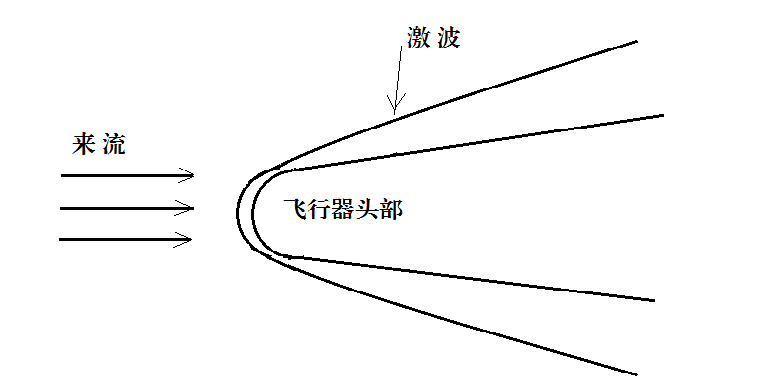
\includegraphics[width=0.75\linewidth]{jibo.png}
\caption{高超声速下的激波示意图}
\label{fig:jibo}
\end{figure}

在超高音速飞行状态下,空气流场会在飞行器的周围形成激波,如图\ref{fig:jibo}所示,激波与壁面之间的流体称为激波层,飞行器壁面附近以及激波后的流场温度大大升高,过高的温度就会引发空气的电离分解现象,使该处物质状态发生本质改变。事实上当空气温度超过800K时,此时的空气已经无法再应用之前的完全气体假设理论了,定容比热、定压比热都将变成与介质温度有关的变量,如果温度超过2000K,氧分子就开始离解,超过4000K氮气开始离解,温度超过9000K后气体原子发生电离,该处流场介质将会变成等离子体,产生如Anderson所说的真实气体效应\cite{anderson1989,lihuiping2010,xiezhixue2011},这种情况下对流场的研究必须考虑化学反应等的影响,并且完全气体中的比热比常数$\gamma=1.4$不再成立。

根据气体动力学中斜激波的理论描述,激波层往往是一个很薄的薄层,激波后面的气体密度会随着来流速度的增大而增大,并且激波形状往往很接近飞行器的外在形状。如果我们假设来流沿x方向流动,通过等熵关系以及理想气体状态方程可以得到如下的关系表达式:
\begin{equation}
\left\{
\begin{aligned}
\frac{\text{d}p}{p}&=-\gamma\cdot u_\infty^2\cdot\frac{\text{d}u}{u}\\
\frac{\text{d}T}{T}&=-(\gamma-1)\cdot u_\infty^2\cdot\frac{\text{d}u}{u}\\
\frac{\text{d}\rho}{\rho}&=-u_\infty^2\cdot\frac{\text{d}u}{u}
\end{aligned}\right.
\label{eq:feixianxing}
\end{equation}
式中,$u_\infty$为来流速度,$p,T,\rho,u,\gamma$分别为压强、温度、密度、速度以及气体比热比。

从流动方程等构成的方程组\eqref{eq:feixianxing}可以看出在高超声速条件下,很小的速度扰动也会引起流场压强等物理量发生巨大的变化,对此就不能如前文那样对方程线性化而忽略微小扰动,计算时必须考虑微小扰动情况,这种非线性性质增大了对高超声速流场的研究难度,但是随着来流速度的增加,激波会越来越贴近飞行器表面,马赫角越来越小,使一些气动力学的问题相对简化。

一般在高超声速下运行的飞行器都会做成钝状的头部外型,这是由于激波会引起流体的熵增,头部温度较高,而在头部的曲率半径的平方与驻点的对流传热是反比关系,因此钝状头部能够有效减轻热载荷。在边界层内,粘性效应降低了流体运动速度,将部分动能转化为内能,从而产生热效应,高超声速中边界层厚度较大,对外部无粘流动干扰较大,同时会影响增加飞行器壁面的阻力以及传热系数。另外当代的高超声速飞行器往往会在海拔很高的高空中飞行,这时该高度周围的空气非常稀薄,分子平均自由程的尺度会接近飞行器本身的尺度,这种情况下无法再用连续方程来描述周围气体特征,并且激波厚度将会有所增加,这种情况可以称之为低密度效应。

从以上分析可以知道由于飞行器周围的流场动能大量转化为激波层内能,引起严重的气动加热,因此在设计高超声速飞行器时,需要对气动加热及热传导系数问题作出预计,进而提出解决办法。热流密度$q_w$一般由以下经验公式给出:
\begin{equation}
q_w=\rho_\infty^N\cdot u_\infty^M\cdot C
\end{equation}
式中,$N,M,C$为与飞行器结构有关的系数,对钝形头部及平板的系数可以参见表\ref{tab:waixingxishu},表中,$R$为钝型头部半径,$h_w$表示实际壁面对应的比焓,$s$为沿壁面距离,$\varphi$为攻角。
\begin{table}[bhtp]
\centering
\caption{不同外型下的经验参数}
\label{tab:waixingxishu}
\begin{tabular}{|c|c|c|c|}
\hline
\diagbox{形状}{系数}&$N$&$M$&$C$\\\hline
钝头&0.5&3.0&$1.83\times10^{-6}R^{-1/2}(1-h_w/h_0)$\\\hline
平板&0.5&3.2&$2.53\times10^{-9}\sin\varphi\sqrt{\cos\varphi}\cdot\sqrt{x}(1-h_w/h_0)$\\\hline
\end{tabular}
\end{table}

从表\ref{tab:waixingxishu}中可以看到当飞行器头部半径小,呈尖型时,头部空气加热率很高,而尖型的外形散热慢导致温度很高,而采用大半径的钝头则有较高的应用价值。另外在飞行器的设计时应该采用耐高温材料,并且可以采用隔热材料或者装置来较少周围流场传递给飞行器的热量。
\section{本章小结}
本章简要介绍了流场运动普遍遵循的流体运动方程,并对流体运动方程组的求解方法作了详细介绍及公式推导,基于favre平均理论,利用大涡模拟及雷诺平均法两种主要模拟方法对流体运动方程组的数值求解,在大涡模拟中使用亚格子模型对滤波后的控制方程求解,具有较高的精度,而在雷诺平均法中主要对$k-\varepsilon$和$k-\omega$二方程模型进行修正得到SST模型进行求解,计算量相对较小且精度较高,最后讨论了在高超声速情况下,流体的结构发生明显变化,空气会发生电离现象,应该考虑到流场的非线性性质 、真实气体效应以及严重的气动加热等问题,并且可以将高超声速飞行器的外形设计为钝头来降低气动加热问题。
